\documentclass[12pt,a4paper]{article}

% Margins.
\setlength{\oddsidemargin}{0in}
\setlength{\evensidemargin}{0in}
\setlength{\headheight}{12pt}
\setlength{\headsep}{42pt}
\setlength{\topmargin}{-54pt}
\setlength{\textwidth}{6.5in}
\setlength{\textheight}{10in}

\usepackage{amsmath}
\usepackage{float}
\usepackage{graphicx}
\usepackage[hyphens]{url}
\usepackage{hyperref}	% Clickable links to figures, references and urls.
\usepackage{datetime}
\usepackage{longtable}
\usepackage{subfigure}

% Links direct to top of figures.
\usepackage[all]{hypcap}

% Drawing.
\usepackage{pgf}
\usepackage{tikz}

% Listings for formatting code.
\usepackage{listings}
\usepackage{textcomp}
% General options.+++
\lstset{breaklines=true, basicstyle=\small\ttfamily, tabsize=4, numbers=left, stepnumber=1, frame=single, showstringspaces=false, upquote=true}
% C++ specific high-lighting. Comments are 50/50 shades of green/black and strings coloured with 60/40 red/black mixture.
\lstset{language=[ISO]C++, commentstyle=\color{green!50!black}, keywordstyle=\color{blue}, stringstyle=\color{red!60!black}}

%opening
\title{\vspace{-3cm}Physics for Engineers\\Class 38\\Induced Electromotive Force ($V_{emf}$)}
\author{Attique Dawood}
\date{November 25, 2013\\[0.2cm] Last Modified: \today, \currenttime}
\begin{document}
\maketitle
\section{Announcements}
\begin{itemize}
\item Expect assignment 09 shortly.
\end{itemize}
\section{Magnetic Flux}
Magnetic flux is given by
\begin{equation}
\psi=\int\limits_{S}\textbf{B}\cdot d{\textbf{S}}.
\end{equation}
Magnetic flux has units Webers. The magnetic flux through a closed surface is zero. This implies that isolated magnetic charge does not exist. Mathematically
\begin{equation}
\oint\limits_{S}\textbf{B}\cdot d{\textbf{S}}=0.
\end{equation}
This is the fourth Maxwell's equation written in integral form.
\section{Induced Electromotive Force}
When a constant current flows in a loop a magnetic field is set up around the loop (Here we refer to 
\textbf{B} as magnetic field). This is shown in figure \ref{B-field-loop}. The number of magnetic field lines passing through the loop is the magnetic flux through the loop. In this case 7 lines cut the loop so flux is $7$ Webers.
\begin{figure}[H]
\centering
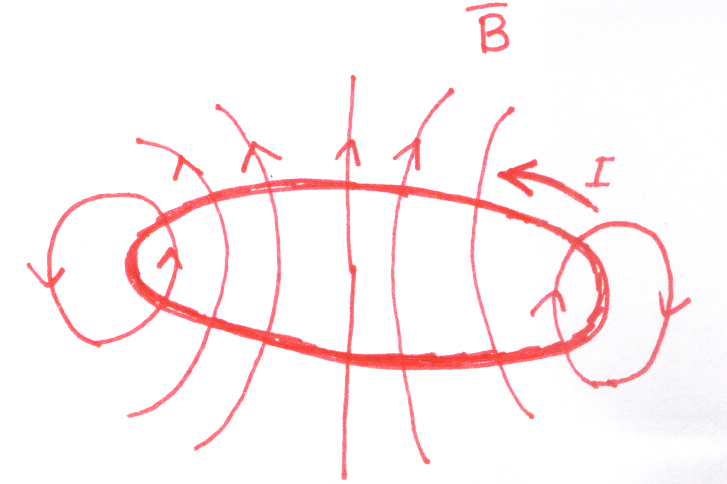
\includegraphics[scale=0.5]{BFieldLoop.png}
\caption{Magnetic field of current carrying loop.}
\label{B-field-loop}
\end{figure}
If we take a loop of wire and move a magnet through it we will notice a current flows through the wire. The current only exists as long as the magnetic is in motion. This experiment can also be performed by keeping magnet still and moving the loop through the magnet as shown in figure \ref{Magnet-through-loop}. 
\begin{figure}[H]
\centering
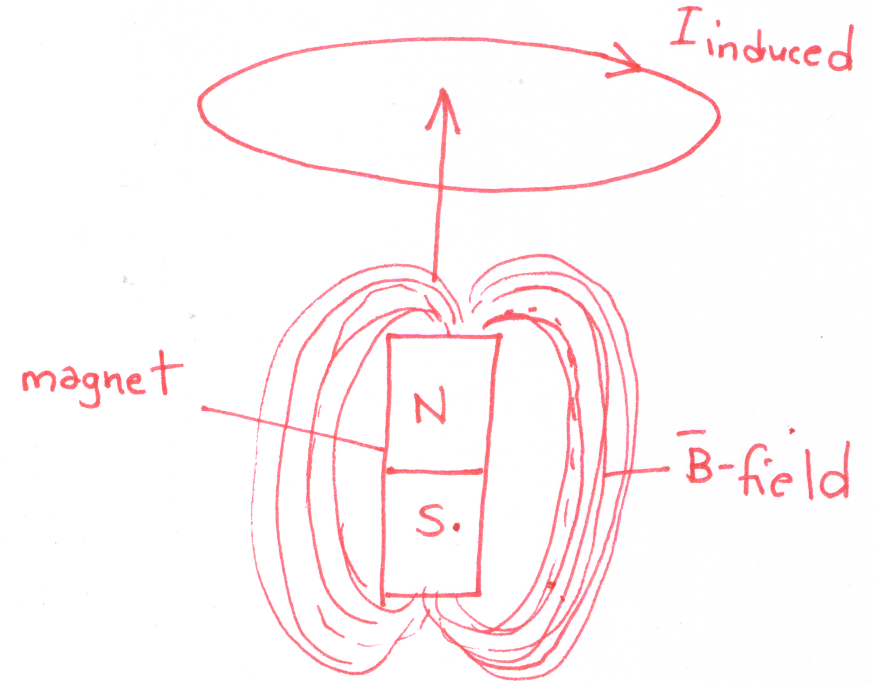
\includegraphics[scale=0.5]{InducedCurrentMagnet.png}
\caption{Magnetic field of current carrying loop.}
\label{Magnet-through-loop}
\end{figure}
So far we have only considered current carrying loops but did not discuss the voltage source that set up that current. Normally we would use a battery and a resistor in series with appropriate values if we want to set up a current $I$ in a loop. The battery is said to provide electromotive force (or emf for short) that keeps current flowing in the loop. The voltage drop across the resistor is $V_R=IR$ as shown in figure \ref{Current-Battery}. We normal don't use the subscript emf in $V_{emf}$ and refer to voltage source as $V$.
\begin{figure}[H]
\centering
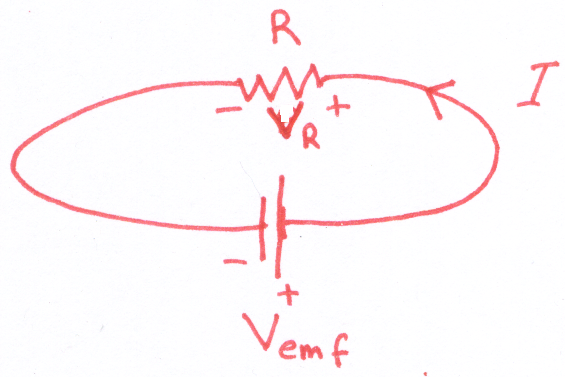
\includegraphics[scale=0.5]{CurrentBattery.png}
\caption{Current set up in a loop due to a voltage source.}
\label{Current-Battery}
\end{figure}
\newpage
Now consider the case we moved the magnet through the loop to set up induced current in the coil. \textbf{There was no battery present so the electromotive force was provided by the changing magnet field}. This emf responsible for setting up induced current is known as induced emf as shown in figure \ref{Induced-emf}.
\begin{figure}[H]
\centering
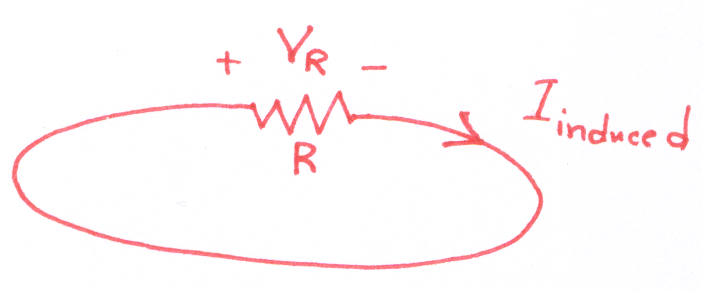
\includegraphics[scale=0.5]{InducedEMF.png}
\caption{Induced current due to induced emf.}
\label{Induced-emf}
\end{figure}
The magnitude of induced emf is equal the rate change of magnetic flux cutting through the loop. Mathematically
\begin{equation}
V_{emf}=-\dfrac{d\Phi_B}{dt}
\end{equation}
\section{Lenz's Law}
Lenz's Law states that induced current will oppose and try to cancel the magnetic field responsible for induced emf. Imagine induced current setting up a magnetic field opposite to the original magnetic field.
\section{Faraday's Law}
What happens if you apply KVL on loop shown in figure \ref{Induced-emf}? KVL around the loop is non--zero! Electric field responsible for induced emf is not conservative. As it happens we need to modify one of our Maxwell's equation and apply a correction.
\begin{equation}
\oint\limits_{L} \textbf{E}\cdot d\textbf{\textit{l}}=-V_{emf}.
\end{equation}
The standard form better known as the Faraday's Law of Induction is
\begin{equation}
\oint\limits_{L} \textbf{E}\cdot d\textbf{\textit{l}}=-\dfrac{d\Phi_B}{dt}.
\end{equation}
\newpage
\section{Exercises}
\noindent\textbf{Question 1} Find the magnitude and direction of induced emf in figure shown below. Also find magnitude of induced current if a current limiting resistor of 1 $\Omega$ is used.
\begin{figure}[H]
\centering
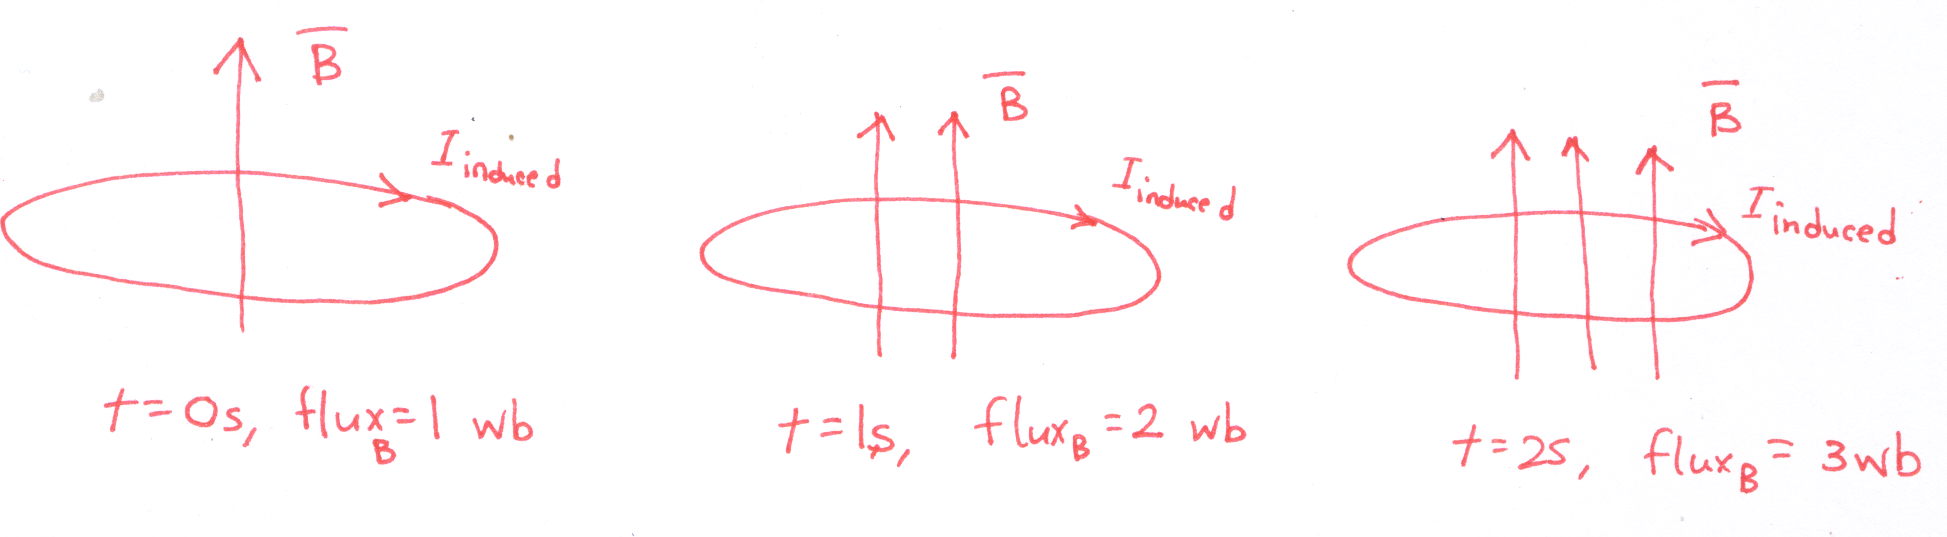
\includegraphics[width=\textwidth]{ChangingFlux.png}
%\caption{Induced current due to induced emf.}
\label{Changing-Flux}
\end{figure}
\noindent\textbf{Question 2} A magnetic field given by $\textbf{B}=10\sin t\hat z$ cuts a current carrying loop. The loop is placed in $xy$--plane centred at $z$--axis and has a radius 5 cm. Find $V_{emf}$ and direction of induced current. What is induced current if current limiting resistor is 1 $\Omega$?
%\noindent\textbf{Question 2 \cite[Problem 7.21, page 300]{Sadiku}} An infinitely long filamentary wire carries 2 A current in $+z$ direction. Find
%\begin{itemize}
%\item[a.] \textbf{B} at (-3, 4, 7)
%\item[b.] Magnetic flux through the surface given by $2<\rho<6$, $0<z<4$ and $\phi=90^0$.
%\end{itemize}
%\nocite{*}
\bibliographystyle{plain}
\bibliography{PhysicsRef}
\end{document}
